\chapter{Conceitos básicos}

\section{Rastreamento}

Segundo \cite{lepetit}, rastrear um objeto é identificar sua posição na cena quando tanto o objeto quanto a câmera estão em movimento. Em outras palavras, é saber a localização de um objeto dada uma entrada em vídeo.

Existem várias formas de rastrear um objeto na cena \cite{teichrieb2007survey} e entre elas existe o rastreamento baseado em modelo e o \emph{Structure from Motion} (\emph{SfM}).

O rastreamento baseado em modelo é caracterizado pelo uso de um modelo 3D pré-definido do objeto a ser rastreado. O modelo serve principalmente para se ter uma estimativa inicial do que vai ser rastreado.
% Existem várias formas de rastrear um objeto na cena \cite{teichrieb2007survey} e uma delas é o rastreamento baseado em modelo. Este tipo de rastreamento é caracterizado pelo uso de um modelo 3D pré-definido do objeto a ser rastreado. Este modelo serve principalmente para se ter uma estimativa inicial do que vai ser rastreado.

Na técnica baseada em \emph{Structure from Motion} (\emph{SfM}) \cite{teichrieb2007survey} não é necessário um conhecimento prévio da cena e, por isso, é bastante útil quando o ambiente a ser rastreado é desconhecido.

Ao se comparar as duas técnicas pode-se dizer que a baseada em modelos é mais eficiente que a \emph{SfM} \cite{drummondecipolla}. A \emph{SfM} baseia-se na análise de todo o frame da sequência de vídeo para poder identificar um movimento na câmera e sabendo-se que poucos segundos de um vídeo pode conter bastante informação, essa análise pode se mostrar lenta. A técnica baseada em modelos, por sua vez, pode tirar proveito de um modelo já conhecido do objeto a ser rastreado. Com isso apenas pontos chaves (\emph{features}) precisam ser analisados para o rastreamento.

% Uma outra técnica de rastreamento é a baseada em \emph{Structure from Motion} (\emph{SfM}) \cite{teichrieb2007survey}. Nesta abordagem não é necessário um conhecimento prévio da cena e, por isso, é bastante útil quando o ambiente a ser rastreado é desconhecido. Apesar disso, a \emph{SfM} tem a desvantagem de ser bastante complexa e não tão eficiente para rastrear uma sequência em vídeo. Isso se deve ao fato de um vídeo conter bastante informação, e muitas vezes apenas uma pequena parte disso seria suficiente para rastrear o movimento da câmera \cite{drummondecipolla}. É nesse aspecto que o rastreamento baseado em modelos se destaca, pois são observados apenas pontos chaves da cena (como os contornos do modelo, por exemplo).

\subsection{Rastreamento baseado em modelo}

Ao rastrear utilizando um modelo pré-definido, devemos estabelecer quais \emph{features} serão extraídas para realizar o rastreamento. Na literatura podemos encontrar exemplos de rastreamento utilizando tanto as arestas quanto a textura do modelo. O rastreamento baseado em texturas tenta casar a textura do modelo com a textura do objeto na imagem capturada.% citacao para texture based
% Uma dessas \emph{features} que podem ser usadas é a textura do modelo. O rastreamento baseado em texturas tenta casar a textura do modelo com a textura do objeto na imagem capturada. 

% Infelizmente esta abordagem não tem um bom desempenho com objetos reflexivos, já que isso pode atrapalhar na identificação da textura.% citation needed

Uma outra \emph{feature} que pode ser extraída do modelo são as arestas. Neste caso as arestas do modelo são casadas com pontos de alto contraste da imagem \cite{drummondecipolla}. O rastreamento baseado em arestas será melhor explicado na seção seguinte.

%\subsection{Rascunho}

\section{Rastreamento por arestas}

Nesta seção explicaremos sobre o rastreamento por arestas, em que as arestas do modelo são utilizadas para poder efetuar o casamento com as imagens capturadas. Tendo uma imagem representando o \emph{frame} atual e o modelo da pose anterior, o rastreamento por aresta consiste em extrair as arestas do \emph{frame} atual e tentar fazer associações com as arestas do modelo a fim de que se possa descobrir quais arestas do modelo correspondem com as arestas extraídas da imagem. Tendo essas correspondências, fica mais fácil definir qual o movimento feito pela câmera entre o \emph{frame} anterior (representado pelo modelo) e o \emph{frame} atual (representado pela imagem extraída da câmera).

%Para a extração das arestas da imagem geralmente são utilizados algoritmos de detecção de borda, como o filtro Sobel.
A vantagem dessa técnica é que arestas são relativamente mais fáceis de serem encontradas em uma imagem. Algoritmos para detecção de bordas são abundantes na literatura e já vem sido bastante estudado em processamento de imagens.%citation

\subsection{Técnicas}

Uma das formas de fazer o casamento entre as arestas do modelo e as arestas da imagem é usar o que pode ser chamado de extração explícita das arestas. Utilizando algum algoritmo de detecção de linha, como a transformada de Hough, as arestas da imagem são extraídas para depois serem comparadas com as do modelo na pose anterior. %cite (Hough) [3] em VTetal

% [como funciona?]. Entretanto um dos problemas desse método é a possibilidade de parte de uma aresta visível estar oculta [como mostra a figura, retirada de \cite{drummondecipolla}]. Isso pode ser interpretado pelo algoritmo como duas arestas menores e que possivelmente não vai ser casada com a aresta correspondente do modelo.

Outra forma de trabalhar com rastreamento baseado em arestas é utilizando a técnica de amostragem de pontos. Neste caso a aresta do modelo é dividida em partes iguais, chamados de amostras (ou \emph{sample-points}). Cada ponto amostrado é então comparado com pontos de forte gradiente da imagem que estão próximos da aresta. Uma das formas de fazer isso é fazer uma busca na direção normal da aresta que passa pelo ponto amostrado. O primeiro ponto de forte gradiente encontrado pode então ser considerado correspondente ao ponto amostrado. Ou seja, é possivelmente onde aquele ponto da pose anterior está no \emph{frame} atual.

% que serão utilizados para casar com as amostras extraídas da imagem.

Em outras palavras o casamento das amostras do modelo com os pontos extraídos da imagem acontece da seguinte forma: primeiro o modelo do \emph{frame} anterior é renderizado a fim de ter uma estimativa inicial da posição do objeto no frame atual; Para cada aresta do modelo são extraídos $N$ amostras que posteriormente serão comparadas com a imagem obtida do frame atual; Em cada amostra do modelo é feita uma busca na normal da aresta a fim de encontrar pontos de forte gradiente (bordas), o que podemos supor que são pontos da aresta da imagem. A partir do casamento das amostras do modelo com os pontos de forte gradientes da imagem, pode ser feita uma estimativa do movimento da câmera.

A extração explícita das arestas tem a vantagem de ser mais robusta, porém é restrita apenas a objetos poligonais. A amostragem de pontos, por sua vez, mostra-se bastante útil quando as arestas não são formadas por retas. Há também a vantagem de trabalhar melhor com arestas oclusas, como mostra a \figref{occlusion}.

\begin{figure}[ht!]
\centering
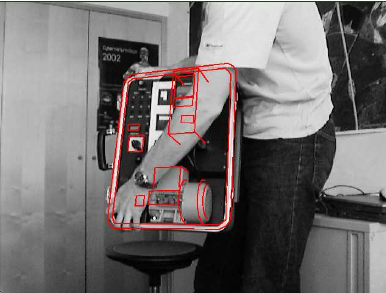
\includegraphics{monografia/occlusion.png}
\caption{Objeto com oclusão parcial das arestas. Imagem retirada de \cite{wuest}}
\label{occlusion}
\end{figure}

Na primeira técnica a aresta parcialmente oclusa seria considerada duas arestas diferentes, enquanto que a amostragem de pontos seria capar de identificá-la como uma aresta só.

\begin{comment}
\subsection{Trabalhando com múltiplas hipóteses}

Algo comum de acontecer na etapa de casamento das amostras do modelo com os pontos de forte gradiente da imagem é que, ao percorrer a normal para achar pontos de forte gradiente, a busca pode retornar mais de um resultado. Ou seja, é possível haver mais de uma hipótese de pontos da imagem para serem casados com uma amostra do modelo. [isso parece ser muito específico]

\subsection{Rascunho}

extração explícita de arestas (ruim por causa da oclusão \cite{drummondecipolla}) \\
amostragem de pontos (sample points. a que eu uso) \\

renderizar o modelo, localizar as arestas visiveis do modelo. a partir dela, extrair sample points. tentar fazer um match das arestas do modelo com as arestas da imagem obtida\cite{drummondecipolla} \\
explicar que pegamos uma aresta do modelo, pegamos alguns sample points. a partir dos sample points seguimos pela normal do ponto e tentamos achar os pontos de forte gradiente. podem existir vários pontos de forte gradiente para um único \emph{sample point} (múltiplas hipóteses) \\

explicar como a escolhas das múltiplas hipóteses podem ser feitas. deixar um gancho para o capítulo seguinte que explica como fazer a escolha utilizando o k-means \\

outliers happens. podem ter outras coisas que formam uma aresta. \\
\end{comment}

\begin{comment}
Em um reprodução de vídeo, rastrear um objeto se caracteriza por identificar a sua posição na cena quando tanto o objeto quanto a câmera está em movimento \cite{lepetit}.

Um vídeo contém bastante informação e é preciso extrair apenas parte dela. Por isso que é usada uma técnica \emph{feature-based}, em que o processamento das imagens é restrito à localização de pontos de forte gradiente como os contornos do objeto \cite{drummondecipolla}.

Uma das formas de efetuar um rastreamento é utilizando um técnica baseada em modelos. Nesse tipo de técnina é necessário um conhecimento prévio do que vai ser rastreado. No caso, é preciso já ter um modelo 3D do objeto a ser rastreado.

* Tipos de rastreamento: SfM, Model based

sfm pega a cena toda.
model based precisa de um modelo 3D pré-construído
    * edge based
        * amostragem de pontos (sample points. é o que eu uso)
        * extração explícita das arestas (ruim por causa da oclusão \cite{drummondecipolla})
    * texture based


model based é mais simples que sfm, mas é preciso ter um modelo de antemão \cite{teichrieb2007survey}

renderizar o modelo, localizar as arestas visiveis do modelo. a partir dela, extrair sample points. tentar fazer um match das arestas do modelo com as arestas da imagem obtida\cite{drummondecipolla}

outliers happens. podem ter outras coisas que formam uma aresta. esse é o problema que eu quero resolver.

Uma das etapas mais importantes de aplicações com realidade aumentada é o rastreamento e registro da cena \cite{teichrieb2007survey}.

Falar sobre o que é rastreamento. Etapas do rastreamento: pegar imagens da camera, identificar?
\end{comment}
